\documentclass{beamer}
\usepackage{beamerthemesplit}
\usepackage{graphicx}
\usepackage{listings}

\title{dnode}
\subtitle{remote execution in the kingdom of node.js}
\author{James Halliday (substack)}
\date{\today}

\begin{document}

\frame{\titlepage}

\frame{
    \frametitle{King Ryan}
    \begin{columns}[c]
    \column{.5\textwidth}
        
\includegraphics[scale=0.8]{images/king_ryan.png}
    \column{.5\textwidth} 
        Ryan decrees
        \pause
        \begin{itemize}
        \item Thou shalt have only one thread.
        \pause
        \item Thy IO shalt be asynchronous.
        \end{itemize}
    \end{columns}
}

\frame{
    \frametitle{call remote functions!}
    {
        
\includegraphics[scale=0.8]{images/cups.png}
        
        \vspace{1em}
        
        If only there were an easier way to expose backend code
        \pause
        that complied with the King's wishes.
        \pause
        
        Well there are lots of these actually.
        \pause
        Most of them suck.
    }
}

\frame{
    \frametitle{At a glance}
    {
        dnode gets out of your way
        \pause
        \begin{itemize}
        \item{fundamentally asynchronous}
        \item[]{
            \begin{itemize}
            \item no return values
            \end{itemize}
        }
        \pause
        \item{symmetric}
        \item[]{
            \begin{itemize}
            \item both sides can call the other's methods
            \end{itemize}
        }
        \pause
        \item{abstract}
        \item[]{
            \begin{itemize}
            \item use it on the browser or the server
            \end{itemize}
        }
        \pause
        \item{simple yet powerful semantics}
        \item[]{
            \begin{itemize}
            \item generalized callback wrapping
            \item no implicit return callbacks
            \end{itemize}
        }
        \end{itemize}
    }
}

\frame{
    \frametitle{Zing example server!}
    {
        \lstinputlisting{code/zing/server.js}
    }
}

\frame{
    \frametitle{Zing example client!}
    {
        \lstinputlisting{code/zing/client.js}
        \pause
        \lstinputlisting{code/zing/console}
    }
}

\frame{
    \frametitle{Fuck yeah callbacks}
    {
        \begin{columns}[c]
        \column{.5\textwidth}
        
\includegraphics[scale=0.5]{images/fuck_yeah.png}
        \column{.5\textwidth} 
            \pause
            \begin{itemize}
            \item and now let's do that in the browser
            \end{itemize}
        \end{columns}
    }
}

\frame{
    \frametitle{Retrofitting the server}
    {
        \lstinputlisting{code/browser/server.js}
    }
}

\frame{
    \frametitle{Browser code}
    {
        \small
        \lstinputlisting{code/browser/index.html}
    }
}

\frame{
    \frametitle{It works in the browser! Huzzah!}
    {
        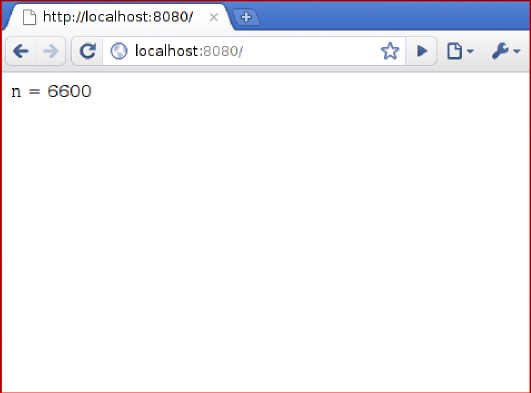
\includegraphics[scale=0.9]{images/browser.png}
    }
}

\frame{
    \frametitle{How it doesn't work}
    {
        \begin{columns}[c]
        \column{.6\textwidth}
            dnode DOESN'T use these
            \begin{itemize}
            \item eval()
            \item Function.prototype.toString()
            \item $<$script$>$ tag injection
            \end{itemize}
        \column{.5\textwidth} 
            
\includegraphics[scale=0.8]{images/no.png}
        \end{columns}
    }
}

\frame{
    \frametitle{How it does work}
    {
        When a function gets called...
        
        \begin{itemize}
        \item{a recursive walk pulls out all the functions from the arguments}
        \item{function paths and IDs sent alongside}
        \item{handles cycles too}
        \end{itemize}
        
        \pause
        \small
        \lstinputlisting{code/protocol_message.json}
        \normalsize
        
        \pause
        This transformation is recursive!
    }
}

\frame{
    \frametitle{It's callbacks all the way down!}
    {
        \lstinputlisting{code/turtles.js}
        
\includegraphics[scale=0.5]{images/thomas_turtle.png}
    }
}

\frame{
    \frametitle{OOP javascript style}
    {
        \lstinputlisting{code/objects.js}
    }
}

\frame{
    \frametitle{Good news for you!}
    {
        \begin{columns}[c]
        \column{.5\textwidth} 
            No need to write your own
            \begin{itemize}
            \item{method dispatcher}
            \item{state machine}
            \item{serialization protocol}
            \end{itemize}
        \column{.5\textwidth}
            
\includegraphics[scale=0.8]{images/robot_stare.png}
        \end{columns}
    }
}

\frame{
    \frametitle{Git it!}
    {
        \begin{center}
        \huge
        github.com/substack/dnode
        
        \vspace{2em}
        
        github.com/substack/dnode-slides
        
        \vspace{2em}
        
        substack.net
        
        \end{center}
    }
}

\end{document}
